\documentclass[11pt,a4paper]{article}
\usepackage[margin=24mm]{geometry}
\usepackage[T1]{fontenc}
\usepackage{lmodern,amsmath,amssymb,amsthm,mathtools,booktabs,array,graphicx,microtype,enumitem,fancyhdr}
\usepackage[dvipsnames]{xcolor}
\usepackage[colorlinks=true,linkcolor=MidnightBlue,urlcolor=MidnightBlue,citecolor=MidnightBlue]{hyperref}
\usepackage{bookmark}
\setlength{\parskip}{5pt}\setlength{\parindent}{0pt}
\setlist{itemsep=3pt,topsep=4pt}
\pagestyle{fancy}\fancyhf{}
\fancyhead[L]{\small Astra P1 | Quantum experimental access}
\fancyhead[R]{\small 5 November 2026}\fancyfoot[C]{\thepage}\setlength{\headheight}{14pt}
\newtheorem{theorem}{Theorem}\newtheorem{corollary}[theorem]{Corollary}
\newcommand{\id}{\operatorname{id}}\newcommand{\Tr}{\operatorname{Tr}}\newcommand{\Ad}{\operatorname{Ad}}
\newcommand{\norm}[1]{\left\lVert #1\right\rVert}
\newcommand{\ket}[1]{\lvert #1\rangle}\newcommand{\bra}[1]{\langle #1\rvert}
\newcommand{\calN}{\mathcal N}\newcommand{\calU}{\mathcal U}\newcommand{\calV}{\mathcal V}
\newcommand{\calK}{\mathcal K}\newcommand{\calP}{\mathcal P}\newcommand{\calZ}{\mathcal Z}\newcommand{\calG}{\mathcal G}
\begin{document}
\begin{titlepage}
\vspace*{14mm}{\Large\color{MidnightBlue} ASTRA P1 SCIENTIFIC RETURN\par}
\vspace{10mm}{\huge\bfseries A physical access theorem\newline for quantum experiments\par}
\vspace{5mm}{\Large Local interaction order, hidden dephasing,\newline and the cost of learning global coherence\par}
\vspace{10mm}{\large 5 November 2026, Australia/Brisbane\par}\vspace{12mm}
\textbf{Selected destination.} Determine whether an arbitrarily powerful, protected quantum computer can efficiently learn global properties of an initially unencoded experiment through weak interactions acting on only a few source qubits at once.

\textbf{Completed result.} A time-uniform acquired-channel contraction theorem derived from simultaneous continuous control and inaccessible dephasing. It gives exponential copy lower bounds for global coherence and worst-case constant-gap purity testing; a polynomial protocol for fixed-weight properties; and an explicit separation when native extensive source interactions are supplied.

\textbf{Evidence status.} Analytic derivation, independent constructive proof audit, and finite-model numerical falsification checks. Historical priority is not established. This is a theoretical access hierarchy, not a demonstrated device or a claim that a civilisation-changing technology has been built.

\vfill The accompanying package contains this manuscript, verification code and results, a scaling figure, and independent companion constructions. The companions are not premises of the main theorem.
\end{titlepage}

\begin{abstract}
An unencoded $n$-qubit source experiences actual inaccessible noise $\lambda\sum_i\mathcal D[Z_i]$. All retained non-Hamiltonian operations preserve the source $Z$-parity sectors. Every remaining Hamiltonian term noncommutes with at most $k$ source $Z_i$, with summed term-norm budget $\Omega$ per source site. The receiver may have arbitrary protected memory, shared ancillas, computation, classical feedback and collective decoding. For $\Omega<2\lambda$, the complete acquired channel contracts a transverse sector of weight $w$ by at most $x_k^w$, where $x_k=\max_{1\le j\le k}(\Omega/(2\lambda j))^{1/j}<1$. For $\Omega\le\lambda$, this is $(\Omega/(2k\lambda))^{w/k}$. A finite Duhamel recursion pays hidden dephasing while each coherence remains unresolved; no initial noise layer is assumed before control.

The theorem implies exponentially many copies for fixed-$k$ global-parity readout and for distinguishing a GHZ state from its classical mixture. Any $k=o(n)$ gives superpolynomial worst-case purity-testing cost at fixed $\Omega/\lambda\le1$. Conversely, explicit finite-slew local meters acquire fixed-weight Pauli properties with polynomial work. A native $n$-body meter reads the particular global coherence with polynomial copies under the same strength and slew scales. Its extensive interaction is an explicitly different physical resource.
\end{abstract}
\tableofcontents\newpage

\section{Scientific decision and inherited machinery}

The capability of interest is a quantum computer that learns useful facts from real quantum experiments. Its computational power does not establish that the relevant experimental information can be acquired before hidden noise removes it.

The inherited resource law limits high-fidelity transfer of an initially unencoded unknown state. It does not by itself settle scientific inference: a state can be impossible to reconstruct while a particular observable remains easy to measure. The new question therefore concerns acquisition of specified scientific information.

Astra's finite causal collector retains its stated assumptions: actual calibrated pure vacuum ports, lossless coherent delivery, a known finite-dimensional source, programmable receiver matrices, and costs dense in source dimension. The separate extreme-channel result concerns the whole finite mixed bath. Neither makes an inaccessible dephasing record observable \cite{astra1732,astra1733}. The prepare-entanglement-first communication operation supplied in the handoff remains valid with its different input timing; it does not eliminate the exposure of an unknown experimental payload already present at the source.

The principle developed here is task dependent: \emph{the order of source coherence to be acquired, and how many source sites a paid interaction can address simultaneously, impose an information-access cost that downstream computing cannot remove.}

\section{Exact access model}
\label{sec:model}

The source is $S=(\mathbb C^2)^{\otimes n}$. The apparatus $A$ includes all accessible quantum memories, controllers and output records. Receiver ancillas may be arbitrarily entangled among themselves, but operationally start independently of the unknown source. Define
\begin{equation}
\calZ_i(X)=(Z_i\otimes I_A)X(Z_i\otimes I_A),\qquad
\mathcal L_{\rm hid}=\lambda\sum_i(\calZ_i-\id),\quad\lambda>0.
\end{equation}
A component odd under one $\calZ_i$ therefore decays at rate $2\lambda$.

The finite-time joint dynamics have generator
\begin{equation}
\mathcal L_t=\mathcal L_{\rm hid}+\calG_t+\sum_a\calK_a(t),\qquad
\calK_a(t)(X)=-i[H_a(t),X].
\end{equation}
The background $\calG_t$ generates completely positive trace-preserving evolution and commutes with every source $\calZ_i$. This restriction applies to the \textbf{full retained operation}, including every accessible field, measurement outcome and feedback record. It is sufficient that all other source Kraus operations commute with the relevant $Z_i$. Receiver-only operations are unrestricted.

Each paid Hamiltonian term has a source commutation support $B_a$:
\begin{equation}
[H_a(t),Z_i\otimes I_A]=0\ (i\notin B_a),\qquad |B_a|\le k.
\end{equation}
Ordinary interactions involving at most $k$ source qubits satisfy this. Arbitrarily extensive diagonal dependence on other source $Z_i$ is also permitted. The receiver part of a term can act on an arbitrarily large protected register. Charge
\begin{equation}
h_a(t)=2\norm{H_a(t)},\qquad
\sum_{a:i\in B_a}h_a(t)\le\Omega\quad\text{for each }i,t.
\label{eq:budget}
\end{equation}
The norm is the operator norm on the joint system.

\textbf{This is an additional locality-resolved assumption.} A bound on $\norm{[H,Z_i]}$ for the total Hamiltonian does not automatically imply \eqref{eq:budget}; cancellations can matter. The actual decomposition and summed strengths are charged. Classical measured feedback may obey the budget separately in every retained branch, as proved below. Coherent control uses the global operator-norm budget.

At the end the source is unavailable and discarded. All outputs, heralding flags and later processing belong to the acquired channel. A final uncharged noncommuting source measurement is not allowed. The hidden-noise record is never accessible. The lower bound grants ideal receiver computation and arbitrary finite acquisition time; adding receiver imperfections cannot improve it.

\section{Acquired-channel contraction theorem}

For $R\subseteq\{1,\ldots,n\}$ define
\begin{equation}
\calP_R=\prod_{i\in R}\frac{\id-\calZ_i}{2}.
\end{equation}
This projection retains operators odd under every $Z_i$ in $R$ and has diamond norm at most one. Products of $X$ and $Y$ on $R$, and GHZ off-diagonal coherence on $R$, lie in this sector. The proof can regard the acquired map as acting on joint $SA$ operators; initializing the apparatus in a fixed input-independent state restricts it to the operational source channel.

\begin{theorem}[Interaction order limits acquired coherence]
\label{thm:main}
Let $\calN$ be an acquired channel in Section~\ref{sec:model}, including source trace and all receiver postprocessing. Put
\begin{equation}
r=\frac{\Omega}{2\lambda},\qquad x_k=\max_{1\le j\le k}\left(\frac rj\right)^{1/j}.
\end{equation}
If $0<r<1$, then for every set $R$ of size $w$,
\begin{equation}
\boxed{\norm{\calN\calP_R}_\diamond\le f_w:=\min\{r^{\lceil w/k\rceil},x_k^w\}.}
\label{eq:main}
\end{equation}
Set $f_0=1$. If $0<\Omega\le\lambda$, the discrete maximum is at $j=k$, giving
\begin{equation}
\boxed{\norm{\calN\calP_R}_\diamond\le\left(\frac{\Omega}{2k\lambda}\right)^{w/k}.}
\label{eq:simple}
\end{equation}
These bounds are uniform in acquisition time, receiver dimension, collective processing and entangled references.
\end{theorem}

\subsection{Proof by a finite unresolved-set recursion}

Write $\calU(T,t)$ for the full propagator and $\Pi$ for source trace followed by any final trace-preserving receiver map. Fix nonempty $R$. Remove every Hamiltonian term touching $R$ and denote the remaining propagator by $\calV_R(u,t)$. It remains completely positive and trace preserving. All remaining dynamics preserve the relevant source parities, so
\begin{equation}
\calV_R(u,t)\calP_R=e^{-2\lambda|R|(u-t)}\widetilde{\calV}_R(u,t)\calP_R,
\quad\norm{\calV_R(u,t)\calP_R}_\diamond\le e^{-2\lambda|R|(u-t)}.
\label{eq:free}
\end{equation}
Here $\widetilde{\calV}_R$ omits hidden noise on $R$ and is also a completely positive trace-preserving propagator. Moreover
\begin{equation}
\Pi\calV_R(T,t)\calP_R=0,
\end{equation}
because source trace annihilates any operator odd under one of its $Z_i$.

The exact Duhamel identity at the first insertion touching $R$ is
\begin{equation}
\Pi\calU(T,t)\calP_R=
\sum_{a:B_a\cap R\ne\varnothing}\int_t^T
\Pi\calU(T,u)\calK_a(u)\calV_R(u,t)\calP_R\,\mathrm du.
\label{eq:duhamel}
\end{equation}
The insertion commutes with $\calP_{R\setminus B_a}$. Insert that projection before the future full propagator and define $F_R(t)=\norm{\Pi\calU(T,t)\calP_R}_\diamond$. Using $\norm{\calK_a}_\diamond\le h_a$ yields
\begin{equation}
F_R(t)\le\sum_{a:B_a\cap R\ne\varnothing}\int_t^T
h_a(u)e^{-2\lambda|R|(u-t)}F_{R\setminus B_a}(u)\,\mathrm du.
\label{eq:recursion}
\end{equation}
Every unresolved set on the right is smaller. All dynamics on already resolved sites, and all receiver processing, remain inside full completely positive contractions. There is no unsigned infinite Dyson expansion growing with total acquisition time.

Induct on $|R|$, with $F_\varnothing\le1$. Let $j_a=|B_a\cap R|$. Since $x_k^{-j}/j\le1/r$ and the resource budget implies $\sum_a j_a h_a(u)\le\Omega|R|$,
\begin{equation}
\sum_a h_a(u)x_k^{-j_a}\le\frac{\Omega|R|}{r}=2\lambda|R|.
\end{equation}
Substitute $F_{R\setminus B_a}\le x_k^{|R|-j_a}$ into \eqref{eq:recursion} to obtain
\begin{equation}
F_R(t)\le x_k^{|R|}\int_t^T2\lambda|R|e^{-2\lambda|R|(u-t)}\,\mathrm du\le x_k^{|R|}.
\end{equation}
The other bound follows by $\sum_a h_a\le\Omega|R|$ and the fact that each insertion removes at most $k$ sites, giving one factor $r$ per resolution step. For $r\le1/2$, $(r/2)^{1/2}\ge r$ and $(r/j)^{1/j}$ increases for real $j\ge2$; hence the discrete maximum is at $k$. This proves the theorem.\qed

\subsection{Retained records and classical feedback}

Covariance of an averaged source channel is insufficient. For example, measuring source $X$ and retaining its outcome reads transverse information at zero charged Hamiltonian strength, while its averaged source channel $(\rho+X\rho X)/2$ commutes with $\Ad_Z$. The full retained instrument fails the required covariance. This counterexample is why the access contract includes every accessible record.

For genuine measured feedback, use the classical-record direct-sum algebra. An operator has blocks $X_m$ and norm $\sum_m\norm{X_m}_1$. Apply the future induction separately to each record and term. In every block,
\begin{equation}
\sum_a h_a(m,t)x_k^{-|B_a(m,t)\cap R|}
\le r^{-1}\sum_a |B_a(m,t)\cap R|h_a(m,t)\le2\lambda|R|.
\end{equation}
Multiply by $\norm{X_m}_1$ and sum. The free evolution is a completely positive contraction on this algebra and retains \eqref{eq:free}. This proves the same theorem under per-record budgets. It does not replace a branchwise bound with a sum of maxima over mutually exclusive outcomes. A coherent controller uses the declared global Hamiltonian decomposition.

\section{Global coherence and purity-testing consequences}

\subsection{Readout of a known Pauli observable}
Let $P$ be a traceless Pauli observable transverse on $w$ sites, and set
\begin{equation}
\rho_\pm=\frac{I\pm aP}{2^n},\qquad0<a\le1.
\end{equation}
Their difference lies in the relevant sector and has trace norm $2a$, hence
\begin{equation}
\tfrac12\norm{\calN(\rho_+)-\calN(\rho_-)}_1\le a f_w.
\end{equation}
The observable may be known in advance. The difficulty is acquiring its value, not finding which observable to ask about.

For a protocol with at most $M$ fresh copies, change one copy at a time in a hybrid argument. Apply Theorem~\ref{thm:main} to that copy's unresolved sites; all other copies and apparatus are part of the remaining system. This allows joint ingestion, interactions across copies and adaptive control under the same per-physical-site and full-instrument restrictions. Thus
\begin{equation}
\tfrac12\norm{\sigma_+^{(M)}-\sigma_-^{(M)}}_1\le aM f_w.
\end{equation}
Equal-prior discrimination with error at most $\zeta<1/2$ requires
\begin{equation}
\boxed{M\ge\frac{1-2\zeta}{a f_w}.}
\label{eq:copies}
\end{equation}
All heralding outcomes are included. Discarded trials remain consumed experimental copies.

\subsection{A constant purity gap}
Consider
\begin{align}
\rho_{\rm coh}&=\ket{\mathrm{GHZ}_+}\bra{\mathrm{GHZ}_+},\quad
\ket{\mathrm{GHZ}_+}=\frac{\ket{0^n}+\ket{1^n}}{\sqrt2},\\
\rho_{\rm mix}&=\tfrac12(\ket{0^n}\bra{0^n}+\ket{1^n}\bra{1^n}).
\end{align}
Their purities are $1$ and $1/2$. Their difference is
\begin{equation}
\Delta=\tfrac12(\ket{0^n}\bra{1^n}+\ket{1^n}\bra{0^n}),\qquad
\calP_{[n]}\Delta=\Delta,\quad\norm\Delta_1=1.
\end{equation}
The same hybrid argument gives
\begin{equation}
\boxed{M\ge2(1-2\zeta)f_n^{-1}.}
\label{eq:purity}
\end{equation}
A universal purity estimator of additive accuracy strictly below $1/4$ must satisfy this on at least the displayed pair. It is a worst-case statement with a constant purity gap, not a statement about every state's purity.

Ideal joint SWAP testing estimates purity with constant copies at fixed accuracy and confidence. That assumes an acquired ideal joint measurement. For the displayed known GHZ promise, ideal local $X$ measurements also suffice; the obstruction is the noisy physical acquisition of those measurements.

\subsection{Interaction order needed for polynomial sampling}
At fixed $0<\Omega/\lambda\le1$, the lower bound is
\begin{equation}
M\ge2(1-2\zeta)\left(\frac{2k\lambda}{\Omega}\right)^{n/k}.
\end{equation}
It is exponential for fixed $k$, and superpolynomial for every $k(n)=o(n)$. If $k\le\sqrt n$, its logarithm is at least a positive constant times $\sqrt n$. If $k>\sqrt n$ but $n/k\to\infty$, that logarithm is at least $(n/(2k))\log n=\omega(\log n)$.

A uniform polynomial-copy guarantee therefore requires interaction order proportional to the source size, or a change of another premise: protection before exposure, lower hidden noise, stronger paid control, or accessible error records. This is a necessary condition in the stated regime, not a sufficiency theorem for arbitrary extensive couplings.

\section{Explicit finite-slew meters}
\label{sec:meters}

These positive constructions assume the displayed Hamiltonians are actual programmable source interactions. They are not inferred from a reduced generator. Let $P$ be a Hermitian Pauli product transverse on $w\ge1$ sites. Initialize a protected meter qubit in $\ket0$ and apply
\begin{equation}
H(t)=\frac{\omega(t)}2P\otimes Y_A.
\end{equation}
With $\mu=\Tr(P\rho)$, the exact Heisenberg equations for $a=\langle X_A\rangle$ and $b=\langle PZ_A\rangle$ are
\begin{equation}
\dot a=\omega b,\qquad\dot b=-\omega a-2w\lambda b,\qquad a(0)=0,\quad b(0)=\mu.
\label{eq:ode}
\end{equation}
Thus $a(T)=\beta_w\mu$ and the meter implements a noisy binary measurement of $P$.

\subsection{Fixed duration, zero start, bounded strength and slew}
For $0<\Omega\le\lambda$, take
\begin{equation}
T=\lambda^{-1},\qquad\omega(t)=\Omega\lambda\min\{t,T-t\},\quad0\le t\le T.
\end{equation}
The waveform starts and ends at zero, has peak $\Omega/2$, slew at most $\Omega\lambda$, and a constant-length description. These scales do not grow with $w$.

Put $L=w\lambda$ and $\mu=1$. Equation~\eqref{eq:ode} gives the Volterra equation $a=I-Ka$ with
\begin{align}
I(t)&=\int_0^t\omega(u)e^{-2Lu}\,\mathrm du,\\
(Ka)(t)&=\int_0^t\omega(u)\int_0^u e^{-2L(u-v)}\omega(v)a(v)\,\mathrm dv\,\mathrm du.
\end{align}
On the supremum norm,
\begin{equation}
\norm K\le q:=\frac{\Omega^2}{8w\lambda^2}\le\tfrac18,\qquad
I(T)=\frac{\Omega}{4w^2\lambda}(1-e^{-w})^2.
\end{equation}
The inverse $(I+K)^{-1}$ has norm at most $1/(1-q)$, so
\begin{equation}
|a(T)-I(T)|\le\frac q{1-q}I(T).
\end{equation}
Consequently
\begin{equation}
\boxed{\beta_w\ge\frac67\frac{\Omega}{4w^2\lambda}(1-e^{-w})^2\ge\frac{\Omega}{12w^2\lambda}.}
\label{eq:beta}
\end{equation}
The last step uses $18(1-e^{-1})^2>7$.

This is a finite-slew construction, not a strict hard-bandwidth certificate. A specific microscopic port, propagation delay, filter and native interaction require separate acquisition. Exact compact time support and strict spectral band limitation cannot both be assumed.

\subsection{Polynomial acquisition of fixed-weight properties}
Use independent local source-meter couplings with $P_i\in\{X_i,Y_i,Z_i\}$. For $X$ and $Y$, the contrast is at least $\Omega/(12\lambda)$. For $Z$, the contrast is $\sin(\Omega/(4\lambda))$, which exceeds the same conservative bound.

For a list of $M_0$ Pauli expectations of weight at most $w_0$, choose uniformly random local Pauli axes on each fresh copy. For requested support $S$ use
\begin{equation}
\widehat p=\mathbf1\{\text{axes match}\}\frac{3^{|S|}}{\prod_{i\in S}\beta_i}\prod_{i\in S}y_i,
\qquad y_i\in\{\pm1\}.
\end{equation}
It is unbiased and satisfies $\mathbb E\widehat p^2\le(3/\beta_{\min}^2)^{w_0}$. Median-of-means and a union bound give additive error $\varepsilon$ for all requested observables, failure probability at most $\delta$, with
\begin{equation}
\boxed{N=O\!\left[\left(\frac3{\beta_{\min}^2}\right)^{w_0}\varepsilon^{-2}\log\frac{M_0}{\delta}\right].}
\label{eq:shadows}
\end{equation}
This is the ordinary local-shadow statistical construction with explicit physical measurement attenuation \cite{shadows}; no new shadow algorithm is claimed. For fixed $w_0$ and strength ratio, polynomial-size lists have polynomial cost. A polynomial-size list of weight $O(\log n)$ also has polynomial sample cost, although enumerating every such observable is a different computational task.

\subsection{Complete resource and precision statement}
Each snapshot consumes one source copy, up to $n$ fresh protected meter qubits, $n$ parallel bounded couplings of duration $1/\lambda$, and $n$ meter measurements. It produces $O(n)$ classical bits. Direct evaluation costs $O(NM_0w_0)$ arithmetic operations and unprocessed storage $O(Nn)$. With parallel per-site hardware, sequential wall time is
\begin{equation}
O\!\left(N(\tau_{\rm prep}+\lambda^{-1}+\tau_{\rm reset}+\tau_{\rm read})\right),
\end{equation}
plus communication and processing latency. Source preparation is not free.

The axes, strengths and noise rate are known model parameters. Alternatively, estimate contrasts by operating the same apparatus on trusted known calibration states. Precision $|\Delta\beta_i|=O(\varepsilon\beta_{\min}/w_0)$ suffices; independent binary calibration has the corresponding inverse-square sample cost. This requires actual calibration preparations and repeatable operation, not merely fitting a reduced generator.

For independent local implementation errors of diamond size $\nu$, a conservative systematic budget is $w_0\nu\beta_{\min}^{-w_0}$. Taking $\nu=O(\varepsilon\beta_{\min}^{w_0}/w_0)$ suffices. At fixed $w_0$ all these requirements are finite and polynomial. The statement is a specified control-model capability, not a demonstrated laboratory implementation.

\section{An explicit extensive-access separation}

Use the same waveform on the actual interaction $P=X_1\cdots X_n$. Its source interaction order is $n$, while its per-site strength and slew remain the stated constants. Equation~\eqref{eq:beta} gives $\beta_n\ge\Omega/(12n^2\lambda)$. For $\rho_\pm=(I\pm aP)/2^n$, meter expectations are $\pm a\beta_n$. Hoeffding estimation gives error at most $\zeta$ with
\begin{equation}
M\le\left\lceil\frac2{a^2\beta_n^2}\log\frac1\zeta\right\rceil
=O\!\left(\frac{\lambda^2 n^4}{a^2\Omega^2}\log\frac1\zeta\right).
\end{equation}
The GHZ state and mixture have $\langle P\rangle=1$ and $0$, so this meter distinguishes that pair with polynomial copies too. This does not construct a polynomial universal purity estimator for all inputs.

The programme uses one meter qubit, duration $1/\lambda$, peak $\Omega/2$, slew $\Omega\lambda$, and an \emph{actual} $n$-body source coupling. A systematic apparatus bias must be below the signal scale $O(\Omega/(\lambda n^2))$, a polynomial precision requirement. A microscopic realization of the extensive interaction is not supplied. Its synthesis from weak few-site interactions during ongoing source dephasing cannot be treated as a free replacement; it is covered by the converse.

\begin{figure}[ht]\centering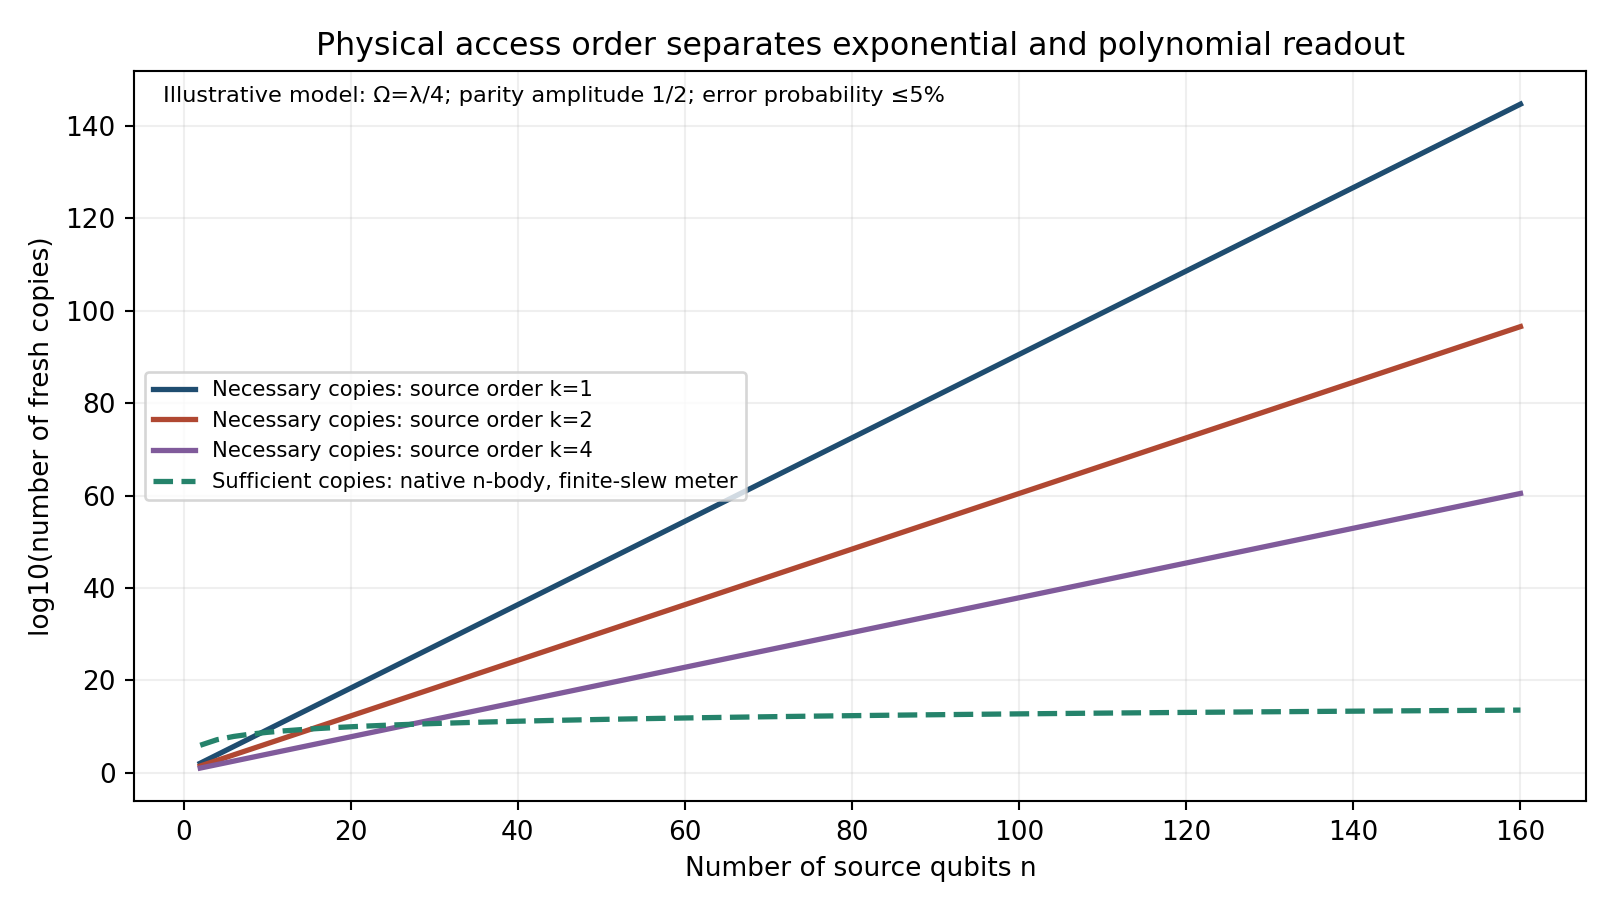
\includegraphics[width=\textwidth]{access_scaling.png}
\caption{Illustrative necessary and sufficient copy budgets for a promised global parity test. Solid curves are lower bounds for small source interaction orders. The dashed curve is a conservative sufficient budget for the explicitly different native $n$-body interface. These are not matched hardware implementations.}\end{figure}

\subsection{The one-copy weak-control power is attained}
For a constant drive on a block of $k$ source sites,
\begin{equation}
\beta_k(t)=\frac{\Omega}{q}e^{-k\lambda t}\sinh(qt),\qquad q=\sqrt{k^2\lambda^2-\Omega^2},
\end{equation}
with its continuous limit at $q=0$. As $\Omega/(k\lambda)\to0$,
\begin{equation}
\max_t\beta_k(t)\sim\frac{\Omega}{2k\lambda}.
\end{equation}
For $n=bk$, independent block meters give output trace distance $a\beta_k^b$ on the Pauli-sign pair. Thus the one-copy control-strength power $n/k$ is attained by ordinary block readout. This asymptotic comparison allows nonzero drive at the input time; the triangular construction separately supplies finite-slew readability.

The general sample lower bound is proportional to $f_n^{-1}$, while elementary parity estimation has an upper bound proportional to $\beta_k^{-2b}$. Both are exponential for fixed $k$, but their exponential constants are not proved optimal here.

\section{A heterogeneous interaction-graph certificate}
For hidden rates $\lambda_i>0$ and term caps $h_a=2\sup_t\norm{H_a(t)}$, the proof also gives
\begin{equation}
F(\varnothing)=1,\qquad F(R)=\min\!\left\{1,
\frac{\sum_{a:B_a\cap R\ne\varnothing}h_a F(R\setminus B_a)}{2\sum_{i\in R}\lambda_i}\right\}.
\end{equation}
Induction yields $\norm{\calN\calP_R}_\diamond\le F(R)$. This certificate is computed from the declared hypergraph and bounds, not supplied as a decoder. Naive evaluation uses $2^n$ sets; no efficient general hypergraph algorithm is claimed. Symmetry or fixed-width structure can reduce that cost. The uniform theorem requires no exponential preprocessing.

\section{Strongest ordinary alternatives and novelty boundary}

\textbf{Ordinary source readout and SWAP.} Fast noncommuting measurement or parallel exchange is a strong baseline when genuinely available. Charge its physical action. The theorem does not deny this capability; it limits it in a weak few-site regime. Ordinary block meters already attain the one-copy weak-control exponent.

\textbf{Fault tolerance and offline entanglement.} These protect resources prepared before exposure. Fault-tolerant quantum input/output already formalizes residual input/output noise and composability \cite{ftio}. The present result does not claim that architecture as new. Native pre-encoding changes its initially unencoded premise.

\textbf{Noisy quantum learning.} Cotler, Gong and Kannan establish noise-sensitive learning and purity-testing limitations in noisy-oracle and effective interstitial-noise models \cite{noisylearning}. The increment pursued here is the direct simultaneous-control theorem, with a locality-resolved resource budget and interaction-order separation. An assumed initial noise layer is not interchangeable with every continuously controlled interface. Historical priority of this precise theorem is not established by the search.

\textbf{Local shadows.} The efficient statistical machinery for bounded-weight properties is established \cite{shadows}. The source-side measurement in this report is explicitly constructed and charged.

This is a separation between receiver computing power and physical access, not a computational complexity-class separation or a universal impossibility of quantum scientific advantage.

\section{Validation and remaining limits}

The numerical code checks 24 triangular-meter cases with widths from $1$ to $1000$, and 60 finite source-receiver evolutions with random allowed Hamiltonians, strong commuting background terms and an initially entangled two-qubit receiver. Both full Pauli-sign and GHZ purity-gap differences were tested. All passed. The largest observed trace norm divided by its smaller analytic certificate was approximately $0.223$. The smallest triangular contrast divided by $\Omega/(12w^2\lambda)$ was approximately $1.187$.

These are floating-point falsification checks, not interval certificates, a test of every control, or replacements for the analytic diamond-norm proof. Independent proof audit identified the full-instrument and classical-feedback conditions stated above.

\begin{enumerate}
\item The general useful bound requires $\Omega<2\lambda$; the clean scaling statements use $\Omega\le\lambda$. The value $2\lambda$ is a proof boundary, not an established physical transition. Exponential task bounds at every fixed finite strength ratio remain unproved here.
\item Noise is independent, inaccessible, Markov $Z$ dephasing. Correlated noise, hidden memory, different axes or accessible records require new arguments.
\item Interaction order and summed term norms are actual assumptions; a total commutator bound alone does not imply them.
\item Source inputs are initially unencoded. Offline Bell preparation and native protected subspaces change that premise.
\item Failed trials consume fresh copies. The result is not a repeat-until-success protocol for the same unknown state.
\item The native extensive interaction is supplied in the separation example, not acquired from local hardware. No finite-bandwidth device or economic advantage is claimed.
\item The positive meters require the displayed actual controls and trusted repeatable calibration. They are not a universal service for an arbitrary immutable source.
\item Worst-case purity testing is hard in the stated regime; many structured or low-weight scientific questions remain efficiently accessible.
\end{enumerate}

\section{Preserved companion constructions}
The accompanying independent reset-output decoder converts coherent local depolarizing environments into payload-independent reset/export flags. It tracks an active circuit and reverses its recorded gates after all active wires have been emitted, avoiding dense exponential synthesis for that structured source class. Accessible noncommuting ports are essential, so it does not evade the hidden-noise theorem.

The independent expander companion treats a different question: mixed output streams, the quantum memory needed to preserve their full output, and low-purity probes that certify memory and capacity. It is preserved separately and is not an unproved premise of this report.

The main architectural consequence is precise: in the proved regime, relevant coherence must be protected before exposure, accessed by the requisite source interaction, or acquired at its resulting copy cost. Additional downstream computation alone cannot pay that physical cost.

\begin{thebibliography}{9}
\bibitem{astra1732} Astra Research Knowledge, \href{https://github.com/harjassand/astra-research-knowledge/blob/8457e1084a3bcf3c4f8e3c7e4da9e0f5045a6570/knowledge/current/packets/N1732.json}{governing packet N1732}: finite causal pure-port collection and forgetting transfer. Pinned repository revision \texttt{8457e1084a3b}; the complete revision is encoded in the link and package handoff.
\bibitem{astra1733} Astra Research Knowledge, \href{https://github.com/harjassand/astra-research-knowledge/blob/8457e1084a3bcf3c4f8e3c7e4da9e0f5045a6570/knowledge/current/packets/N1733.json}{governing packet N1733}: whole mixed-bath complement under exact extreme-channel premises, same pinned revision.
\bibitem{noisylearning} J. Cotler, W. Gong and I. Kannan, \emph{Noisy quantum learning theory}, Nature Communications 17, 6979 (2026), DOI 10.1038/s41467-026-73693-x. \href{https://arxiv.org/html/2512.10929v2}{Technical version read: arXiv:2512.10929v2}.
\bibitem{ftio} M. Christandl, O. Fawzi and A. Goswami, \emph{Fault-tolerant quantum input/output}, \href{https://arxiv.org/abs/2408.05260}{arXiv:2408.05260v3} (2025); IEEE Transactions on Information Theory 72, 3098--3128 (2026).
\bibitem{shadows} H.-Y. Huang, R. Kueng and J. Preskill, \emph{Predicting many properties of a quantum system from very few measurements}, Nature Physics 16, 1050--1057 (2020), DOI 10.1038/s41567-020-0932-7. \href{https://arxiv.org/abs/2002.08953}{arXiv:2002.08953}.
\end{thebibliography}
\end{document}
